\section{遞迴}
    \subsection{先說說定義}
    所謂的遞迴就是函數直接或間接的使用自己本身。這樣說不是很清楚,以下引用\textbf{維基百科}作為示例。

    \begin{quoting}
        從前有座山,山裡有座廟,廟裡有個老和尚,正在給小和尚講故事呢!故事是什麼呢?「從前有座山,山裡有座廟,廟裡有個老和尚,正在給小和尚講故事呢!故事是什麼呢?『從前有座山,山裡有座廟,廟裡有個老和尚,正在給小和尚講故事呢!故事是什麼呢?……』」
    \end{quoting}

    實際上,通常遞迴的程式碼都會寫在另一個函式($Function$)裡面。以下用最常見的二階線性遞迴—費氏數列做為一個範例。

    \begin{lstlisting}[caption=費氏數列的範例]
int f(int n){
    if(n==1 || n==2){
        return 1;
    }
    return f(n-1)+f(n-2);
}\end{lstlisting}

    如果你用紙筆執行這段程式碼,你會看到你的$f(n)$不斷的呼叫$f(n-1)$以及$f(n-2)$。例如$f(5)$呼叫$f(4)$與$f(3)$,$f(4)$呼叫$f(3)$與$f(2)$,$f(3)$呼叫$f(2)$與$f(1)$,$f(3)$呼叫$f(2)$與$f(1)$。

    注意這裡的``$f(3)$呼叫$f(2)$與$f(1)$"是刻意重複兩次的,因為他們被不同的$f$呼叫。

    你應該會發現,隨著$n$越來越大,你的程式也會越跑越久。大概到$5,6$十就有點跑不動。然後如果你更聰明,你就會發現你的程式好像不斷在重複做某些事情。如果你發現的話那恭喜你,你已經一腳踏進$DP$的深坑了。

    什麼?!你說你已經會 $DP$ 了,別急後面會有額外的章節討論 $DP$。

    \subsection{實際上用在哪裡}
    在程式競賽上,遞迴主要都用在偷小分數上。但不要小看他,也許會成為你獲勝的關鍵。

    此外,許多圖論演算法會用到,特別是$DFS$。

    \subsection{偷分的暴力遞迴術}

    \example 井字遊戲(110東區模擬賽)

    \textbf{題目敘述}
    
    熟悉博士為了改變未來所以想要預測未來,雖然他知道世界上許多元素現在的狀態,但是他的魔法還不足以運算出所有的可能性,於是他決定從基礎的井字遊戲開始訓練。熟悉博士認為如果能夠預測出井字遊戲的每一種結果,距離預測未來也不遠了吧!井字遊戲作為一個國際雙人競技項目而家喻戶曉,其規則如下:

    \begin{enumerate}
        \item 給予一個大小為 3 × 3 的棋盤,棋盤每格的初始狀態皆為空,且只能夠被填入一個符號。
        \item 兩位玩家分別使用 'o'、'x',輪流把自己所屬的符號填入棋盤中。
        \item 當任一玩家的三個符號在棋盤上連成一條橫、直、或是斜線,該玩家獲勝並遊戲結束。
        \item 如果棋盤每一格都已被填入符號,遊戲結束且兩玩家平手。
    \end{enumerate}

    你身為熟悉博士的頂級隨從 Maowu,不只上知天文下知地理還是個頂尖的 Coder,而熟悉博士有時對自己的預測結果感到不安,於是他請你幫助他驗證答案。
    
    熟悉博士會給你井字遊戲目前的狀態,假設雙方輪流隨機把符號填入,請你告訴熟悉博士所有可能的結果中,使用 'o' 一方贏的次數、使用 'x' 一方贏的次數、以及雙方平手的次數。

    \textbf{輸入說明}

    輸入總共 3 行,每行有 3 個以空白隔開的字元表示給定棋盤的狀態,'-' 表示該格尚未被填入,'o'、'x' 則表示該格已被該方填入。保證輸入棋盤為 'o' 先手且盤面合法。

    \textbf{輸出說明}
    
    輸出共 1 行,包含 3 個整數,分別代表 'o' 一方贏的次數、'x' 一方贏的次數、以及雙方平手的次數,數字之間以空格隔開。

    \textbf{範例測試}

    \begin{tabular}{|m{7cm}|m{7cm}|}
        \hline
        範例輸入 1 & 範例輸出 1 \\
        \hline
        \verb|o - x| &  \verb|1 0 1| \\
        \verb|x o o| &  \\
        \verb|- o x| &  \\
        \hline
        範例輸入 2 & 範例輸出 2 \\
        \hline
        \verb|x o o| &  \verb|2 1 2| \\
        \verb|- - -| &  \\
        \verb|x x o| &  \\
        \hline
    \end{tabular}

    這一題的滿分解就是遞迴,概念是搜尋完所有可能的狀態。這樣解釋不算是非常清楚,我們多額外解釋。首先,我們要一一填滿空的格子,同時,我們知道這個遊戲有可能提早結束。所以應該要在填空之前確認有沒有人贏,接著在所有可能的空格依序選擇要填的下一個,直到填滿為止。

    \begin{lstlisting}[caption=井字遊戲解答]
// 下方程式中,check()會在每次下棋前判斷誰是贏家。 
// -1 表示還沒有結束,0表示'o'贏,1表示'x'贏,2表示平手。
// 
// ttt是主要的遞迴函式,至於裡面的step則是為了判斷輪到誰下棋。

#include<bits/stdc++.h>
using namespace std;

char mp[5][5];
int ct[5];

// 判斷盤面局勢
int check(){
    for(int i=0;i<3;++i){
        // o-- | -o- | --o
        // o-- | -o- | --o
        // o-- | -o- | --o
        if(mp[i][0]==mp[i][1] && mp[i][1]==mp[i][2]){
            if(mp[i][0]=='o'){
                return 0;
            }else if(mp[i][0]=='x'){
                return 1;
            }
        }

        // ooo | --- | ---
        // --- | ooo | ---
        // --- | --- | ooo
        if(mp[0][i]==mp[1][i] && mp[1][i]==mp[2][i]){
            if(mp[0][i]=='o'){
                return 0;
            }else if(mp[0][i]=='x'){
                return 1;
            }
        }
    }
    
    // o-- 
    // -o-
    // --o
    if(mp[0][0]==mp[1][1] && mp[1][1]==mp[2][2]){
        if(mp[0][0]=='o'){
            return 0;
        }else if(mp[0][0]=='x'){
            return 1;
        }
    }

    // --o
    // -o-
    // o--
    if(mp[0][2]==mp[1][1] && mp[1][1]==mp[2][0]){
        if(mp[0][2]=='o'){
            return 0;
        }else if(mp[0][2]=='x'){
            return 1;
        }
    }

    // is tie?
    bool isfull=true;
    for(int i=0;i<3;++i){
        for(int j=0;j<3;++j){
            if(mp[i][j]=='-'){
                isfull=false;
            }
        }
    }

    if(isfull){
        return 2;
    }else{
        return -1;
    }
}

void ttt(int step){
    int ck=check();
    if(ck!=-1){
        ct[ck]++;
        return;
    }

    for(int i=0;i<3;++i){
        for(int k=0;k<3;++k){
            if(mp[i][k]=='-'){
                // 奇數次下一個人是'x'
                if(step&1){
                    mp[i][k]='x';
                }else{
                    mp[i][k]='o';
                }

                ttt(step+1);
                mp[i][k]='-';
            }
        }
    }
}

int main(){
    ios::sync_with_stdio(0);cin.tie(0);

    int step=0;
    for(int i=0;i<3;++i){
        for(int j=0;j<3;++j){
            cin>>mp[i][j];
            if(mp[i][j]!='-') step++;
        }
    }

    ttt(step);
    for(int i=0;i<3;++i){
        cout<<ct[i]<<" ";
    }
    cout<<"\n";
}\end{lstlisting}

    \subsection{範例與練習}

    \problem 火柴棒等式

    \textbf{題目敘述}
    
    給你 $n$ 根火柴棍,你可以拼出多少個形如 $A+B=C$ 的等式?等式中的 $A$、$B$、$C$ 是用火柴棍拼出的整數(若該數非零,則最高位不能是 $0$)。用火柴棍拼數字 $0\sim9$ 的拼法如圖所示:

    
    \begin{figure}[h]
        \centering
        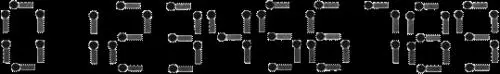
\includegraphics[width=\textwidth]{../Images/Recursive_Torch.png}
    \end{figure}

    \begin{enumerate}
        \item 加號和等號個用掉$2$根火柴。
        \item 如果 $A \ne B$ ,則 $A+B=C$ 與 $B+A=C$ 視為不同的等式。$A,B,C \ge 0$
        \item 火柴要用完。
    \end{enumerate}

    \textbf{輸入說明}

    一個整數 $n, 1 \le n \le 24$。

    \textbf{輸出說明}
    
    一個整數,表示可以拼的等式數目。

    \textbf{範例測試}

    \begin{tabular}{|m{7cm}|m{7cm}|}
        \hline
        範例輸入 1 & 範例輸出 1 \\
        \hline
        \verb|14| &  \verb|2| \\
        \hline
        範例輸入 2 & 範例輸出 2 \\
        \hline
        \verb|18| &  \verb|9| \\
        \hline
    \end{tabular}
    